%%%%%%%%%%%%%%%%%%%%%%%%%%%%%%%%%%%%%%%%%
% University/School Laboratory Report
% LaTeX Template
% Version 3.1 (25/3/14)
%
% This template has been downloaded from:
% http://www.LaTeXTemplates.com
%
% Original author:
% Linux and Unix Users Group at Virginia Tech Wiki 
% (https://vtluug.org/wiki/Example_LaTeX_chem_lab_report)
%
% License:
% CC BY-NC-SA 3.0 (http://creativecommons.org/licenses/by-nc-sa/3.0/)
%
%%%%%%%%%%%%%%%%%%%%%%%%%%%%%%%%%%%%%%%%%

%----------------------------------------------------------------------------------------
%	PACKAGES AND DOCUMENT CONFIGURATIONS
%----------------------------------------------------------------------------------------

\documentclass{article}\usepackage[]{graphicx}\usepackage[]{color}
%% maxwidth is the original width if it is less than linewidth
%% otherwise use linewidth (to make sure the graphics do not exceed the margin)
\makeatletter
\def\maxwidth{ %
  \ifdim\Gin@nat@width>\linewidth
    \linewidth
  \else
    \Gin@nat@width
  \fi
}
\makeatother

\definecolor{fgcolor}{rgb}{0.345, 0.345, 0.345}
\newcommand{\hlnum}[1]{\textcolor[rgb]{0.686,0.059,0.569}{#1}}%
\newcommand{\hlstr}[1]{\textcolor[rgb]{0.192,0.494,0.8}{#1}}%
\newcommand{\hlcom}[1]{\textcolor[rgb]{0.678,0.584,0.686}{\textit{#1}}}%
\newcommand{\hlopt}[1]{\textcolor[rgb]{0,0,0}{#1}}%
\newcommand{\hlstd}[1]{\textcolor[rgb]{0.345,0.345,0.345}{#1}}%
\newcommand{\hlkwa}[1]{\textcolor[rgb]{0.161,0.373,0.58}{\textbf{#1}}}%
\newcommand{\hlkwb}[1]{\textcolor[rgb]{0.69,0.353,0.396}{#1}}%
\newcommand{\hlkwc}[1]{\textcolor[rgb]{0.333,0.667,0.333}{#1}}%
\newcommand{\hlkwd}[1]{\textcolor[rgb]{0.737,0.353,0.396}{\textbf{#1}}}%

\usepackage{framed}
\makeatletter
\newenvironment{kframe}{%
 \def\at@end@of@kframe{}%
 \ifinner\ifhmode%
  \def\at@end@of@kframe{\end{minipage}}%
  \begin{minipage}{\columnwidth}%
 \fi\fi%
 \def\FrameCommand##1{\hskip\@totalleftmargin \hskip-\fboxsep
 \colorbox{shadecolor}{##1}\hskip-\fboxsep
     % There is no \\@totalrightmargin, so:
     \hskip-\linewidth \hskip-\@totalleftmargin \hskip\columnwidth}%
 \MakeFramed {\advance\hsize-\width
   \@totalleftmargin\z@ \linewidth\hsize
   \@setminipage}}%
 {\par\unskip\endMakeFramed%
 \at@end@of@kframe}
\makeatother

\definecolor{shadecolor}{rgb}{.97, .97, .97}
\definecolor{messagecolor}{rgb}{0, 0, 0}
\definecolor{warningcolor}{rgb}{1, 0, 1}
\definecolor{errorcolor}{rgb}{1, 0, 0}
\newenvironment{knitrout}{}{} % an empty environment to be redefined in TeX

\usepackage{alltt}

\usepackage[version=3]{mhchem} % Package for chemical equation typesetting
\usepackage{siunitx} % Provides the \SI{}{} and \si{} command for typesetting SI units
\usepackage{graphicx} % Required for the inclusion of images
\usepackage{natbib} % Required to change bibliography style to APA
\usepackage{amsmath} % Required for some math elements 
\usepackage[table]{xcolor}
\usepackage{colortbl}


\usepackage{geometry}
 \geometry{
 a4paper,
 total={210mm,297mm},
 left=20mm,
 right=20mm,
 top=20mm,
 bottom=20mm,
 }



\setlength\parindent{0pt} % Removes all indentation from paragraphs

\renewcommand{\labelenumi}{\alph{enumi}.} % Make numbering in the enumerate environment by letter rather than number (e.g. section 6)

%\usepackage{times} % Uncomment to use the Times New Roman font

%----------------------------------------------------------------------------------------
%	DOCUMENT INFORMATION
%----------------------------------------------------------------------------------------




\title{Geyser daily report for Sunday, October 11} % Title
%\author{Andrew \textsc{Cloete}} % Author name
\date{\vspace{-5ex}} % Date for the report
\IfFileExists{upquote.sty}{\usepackage{upquote}}{}
\begin{document}

\maketitle % Insert the title, author and date


% If you wish to include an abstract, uncomment the lines below
% \begin{abstract}
% Abstract text
% \end{abstract}

%----------------------------------------------------------------------------------------
%	SECTION 1
%----------------------------------------------------------------------------------------



\section{Overview}



Total hot water used \dotfill  266.8 litres\\
Number of events larger than 10 litres \dotfill 8\\
Number of events smaller than 10 litres \dotfill 15\\
Total number of events \dotfill 23\\

Maximum hot water temperature (geyser setpoint) \dotfill  48.0 $^{\circ}$C\\
Average hot water temperature \dotfill  43.0 $^{\circ}$C\\
Coldest geyser outlet temperature \dotfill  38.0 $^{\circ}$C\\
Average ambient temperature at geyser \dotfill  20.0 $^{\circ}$C\\

Electrical energy consumed \dotfill   12.1 kWh\\
Effective energy consumed \dotfill  8.4 kWh\\
Standing losses \dotfill   3.7 kWh\\
Percentage energy wasted \dotfill   30.6 \%\\
Estimated cost of electricity \dotfill  R 18.15\\
Estimated cost of standing losses \dotfill  R 5.55\\



\section{Other participant comparison}

Your Geyser ID is  \dotfill 106\\




\begin{center}
\begin{knitrout}
\definecolor{shadecolor}{rgb}{0.969, 0.969, 0.969}\color{fgcolor}
\begin{tabular}{l|r|r|r|r|r}
\hline
ID & 104.00 & 106.00 & 107.00 & 109.00 & 112.00\\
\hline
Total Volume (l) & 40.30 & 266.80 & 135.60 & 79.30 & 62.90\\
\hline
Electrical energy (kWh) & 3.60 & 12.10 & 6.60 & 6.70 & 6.90\\
\hline
Effective energy (kWh) & 1.60 & 8.40 & 4.30 & 4.10 & 3.10\\
\hline
Est cost (R) & 5.40 & 18.15 & 9.90 & 10.05 & 10.35\\
\hline
Energy loss (kWh) & 2.00 & 3.70 & 2.30 & 2.60 & 3.80\\
\hline
Loss (\%) & 55.60 & 30.60 & 34.80 & 38.80 & 55.10\\
\hline
Out Min (C) & 41.00 & 38.00 & 39.00 & 60.00 & 37.00\\
\hline
Out Mean (C) & 46.00 & 43.00 & 45.00 & 63.00 & 44.00\\
\hline
Out Max (C) & 54.00 & 48.00 & 52.00 & 69.00 & 62.00\\
\hline
In Min (C) & 16.00 & 13.00 & 13.00 & 18.00 & 12.00\\
\hline
In Mean (C) & 23.00 & 20.00 & 24.00 & 23.00 & 15.00\\
\hline
In Max (C) & 32.00 & 31.00 & 43.00 & 32.00 & 22.00\\
\hline
Amb Min (C) & 14.00 & 13.00 & 12.00 & 18.00 & 11.00\\
\hline
Amb Mean (C) & 20.00 & 20.00 & 24.00 & 24.00 & 17.00\\
\hline
Amb Max (C) & 29.00 & 30.00 & 43.00 & 35.00 & 24.00\\
\hline
Total \#events & 3.00 & 23.00 & 7.00 & 15.00 & 3.00\\
\hline
Large \#events & 1.00 & 8.00 & 3.00 & 2.00 & 1.00\\
\hline
Small \#events & 2.00 & 15.00 & 4.00 & 13.00 & 2.00\\
\hline
Packet loss (\%) & 0.28 & 0.35 & 1.18 & 11.25 & 0.56\\
\hline
\end{tabular}


\end{knitrout}
\end{center}

\newpage
\section{Hot water usage event summary}



\subsection{Large events}

The following is a summary of events \textbf{larger} than 10 litres. \\

Number of events \dotfill 8\\
Total volume of water consumed \dotfill 241.4 litres\\
Total energy consumed \dotfill 7.7 kWh\\
Total estimated cost \dotfill R11.48\\

\begin{center}
\begin{table}[h!]
\begin{knitrout}
\definecolor{shadecolor}{rgb}{0.969, 0.969, 0.969}\color{fgcolor}
\begin{tabular}{l|l|r|r|r|r|r}
\hline
  & Start time & Volume (l) & Duration & Avg temperature & Est energy (kWh) & Est cost (R)\\
\hline
1 & 06:52:39 & 10.63 & 3.00 & 42.33 & 0.32 & 0.48\\
\hline
8 & 09:23:39 & 29.51 & 12.00 & 47.82 & 0.97 & 1.46\\
\hline
12 & 11:02:39 & 16.71 & 4.00 & 47.75 & 0.52 & 0.78\\
\hline
13 & 11:07:39 & 11.54 & 2.00 & 48.00 & 0.38 & 0.56\\
\hline
14 & 11:10:39 & 47.68 & 13.00 & 48.00 & 1.55 & 2.32\\
\hline
16 & 11:30:39 & 38.94 & 11.00 & 47.60 & 1.24 & 1.87\\
\hline
19 & 19:06:39 & 42.27 & 18.98 & 43.32 & 1.23 & 1.84\\
\hline
21 & 20:48:39 & 44.18 & 4.00 & 46.25 & 1.45 & 2.18\\
\hline
\end{tabular}


\end{knitrout}
\caption{List of events larger than 10 litres}
\end{table}
\end{center}


\subsection{Small events}

The following is a summary of events \textbf{smaller} than 10 litres. \\

Number of events \dotfill 15\\
Total volume of water consumed \dotfill 25.3 litres\\
Energy consumed \dotfill 0.8 kWh\\
Estimated cost \dotfill R1.17\\

\begin{center}
\begin{table}[h!]
\begin{knitrout}
\definecolor{shadecolor}{rgb}{0.969, 0.969, 0.969}\color{fgcolor}
\begin{tabular}{l|l|r|r|r|r|r}
\hline
  & Start time & Volume (l) & Duration & Avg temperature & Est energy (kWh) & Est cost (R)\\
\hline
2 & 07:04:39 & 2.82 & 3.00 & 43.67 & 0.09 & 0.13\\
\hline
3 & 07:12:39 & 1.34 & 2.00 & 45.00 & 0.04 & 0.07\\
\hline
4 & 07:30:39 & 0.15 & 1.00 & 45.00 & 0.00 & 0.01\\
\hline
5 & 08:00:39 & 0.29 & 0.98 & 45.00 & 0.01 & 0.01\\
\hline
6 & 09:03:39 & 0.33 & 1.00 & 46.00 & 0.01 & 0.01\\
\hline
7 & 09:20:39 & 0.39 & 0.98 & 45.00 & 0.01 & 0.01\\
\hline
9 & 09:38:39 & 1.22 & 1.00 & 47.00 & 0.04 & 0.06\\
\hline
10 & 09:40:38 & 7.92 & 4.02 & 47.50 & 0.26 & 0.38\\
\hline
11 & 09:47:39 & 1.13 & 2.00 & 47.00 & 0.03 & 0.05\\
\hline
15 & 11:25:39 & 1.13 & 2.00 & 48.00 & 0.03 & 0.05\\
\hline
17 & 13:23:38 & 0.28 & 1.02 & 47.00 & 0.01 & 0.01\\
\hline
18 & 16:52:38 & 3.20 & 1.02 & 45.00 & 0.09 & 0.13\\
\hline
20 & 19:49:39 & 0.12 & 1.00 & 43.00 & 0.00 & 0.01\\
\hline
22 & 21:32:39 & 4.90 & 2.00 & 46.00 & 0.16 & 0.23\\
\hline
23 & 22:07:39 & 0.13 & 1.00 & 44.00 & 0.00 & 0.01\\
\hline
\end{tabular}


\end{knitrout}
\caption{List of events smaller than 10 litres}
\end{table}
\end{center}




\newpage

\section{Graphs}
\begin{knitrout}
\definecolor{shadecolor}{rgb}{0.969, 0.969, 0.969}\color{fgcolor}\begin{figure}[h!]

{\centering 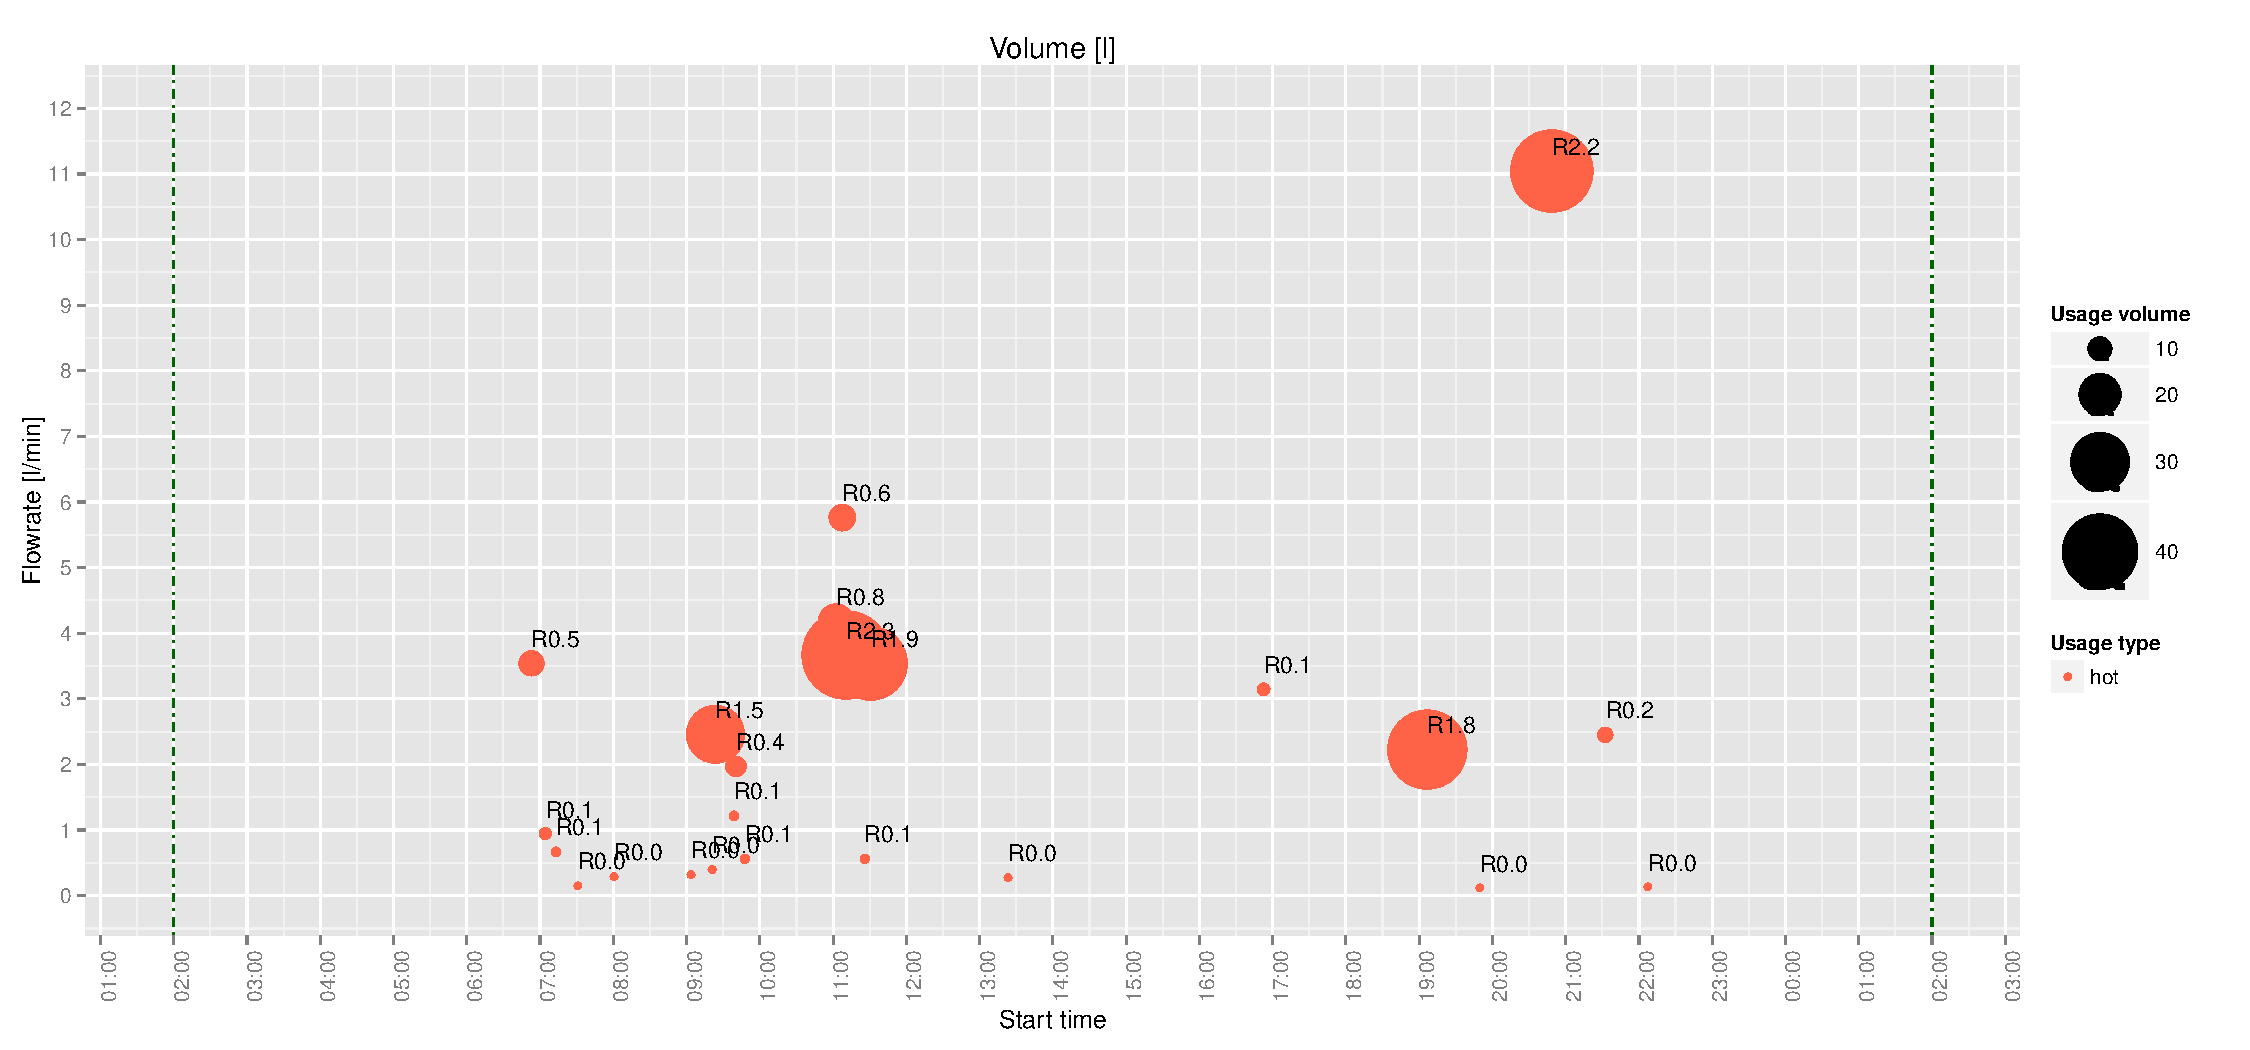
\includegraphics[width=\maxwidth]{figure/balloon-1} 

}

\caption[Usage events and volumes]{Usage events and volumes}\label{fig:balloon}
\end{figure}


\end{knitrout}

\begin{knitrout}
\definecolor{shadecolor}{rgb}{0.969, 0.969, 0.969}\color{fgcolor}\begin{figure}[h!]
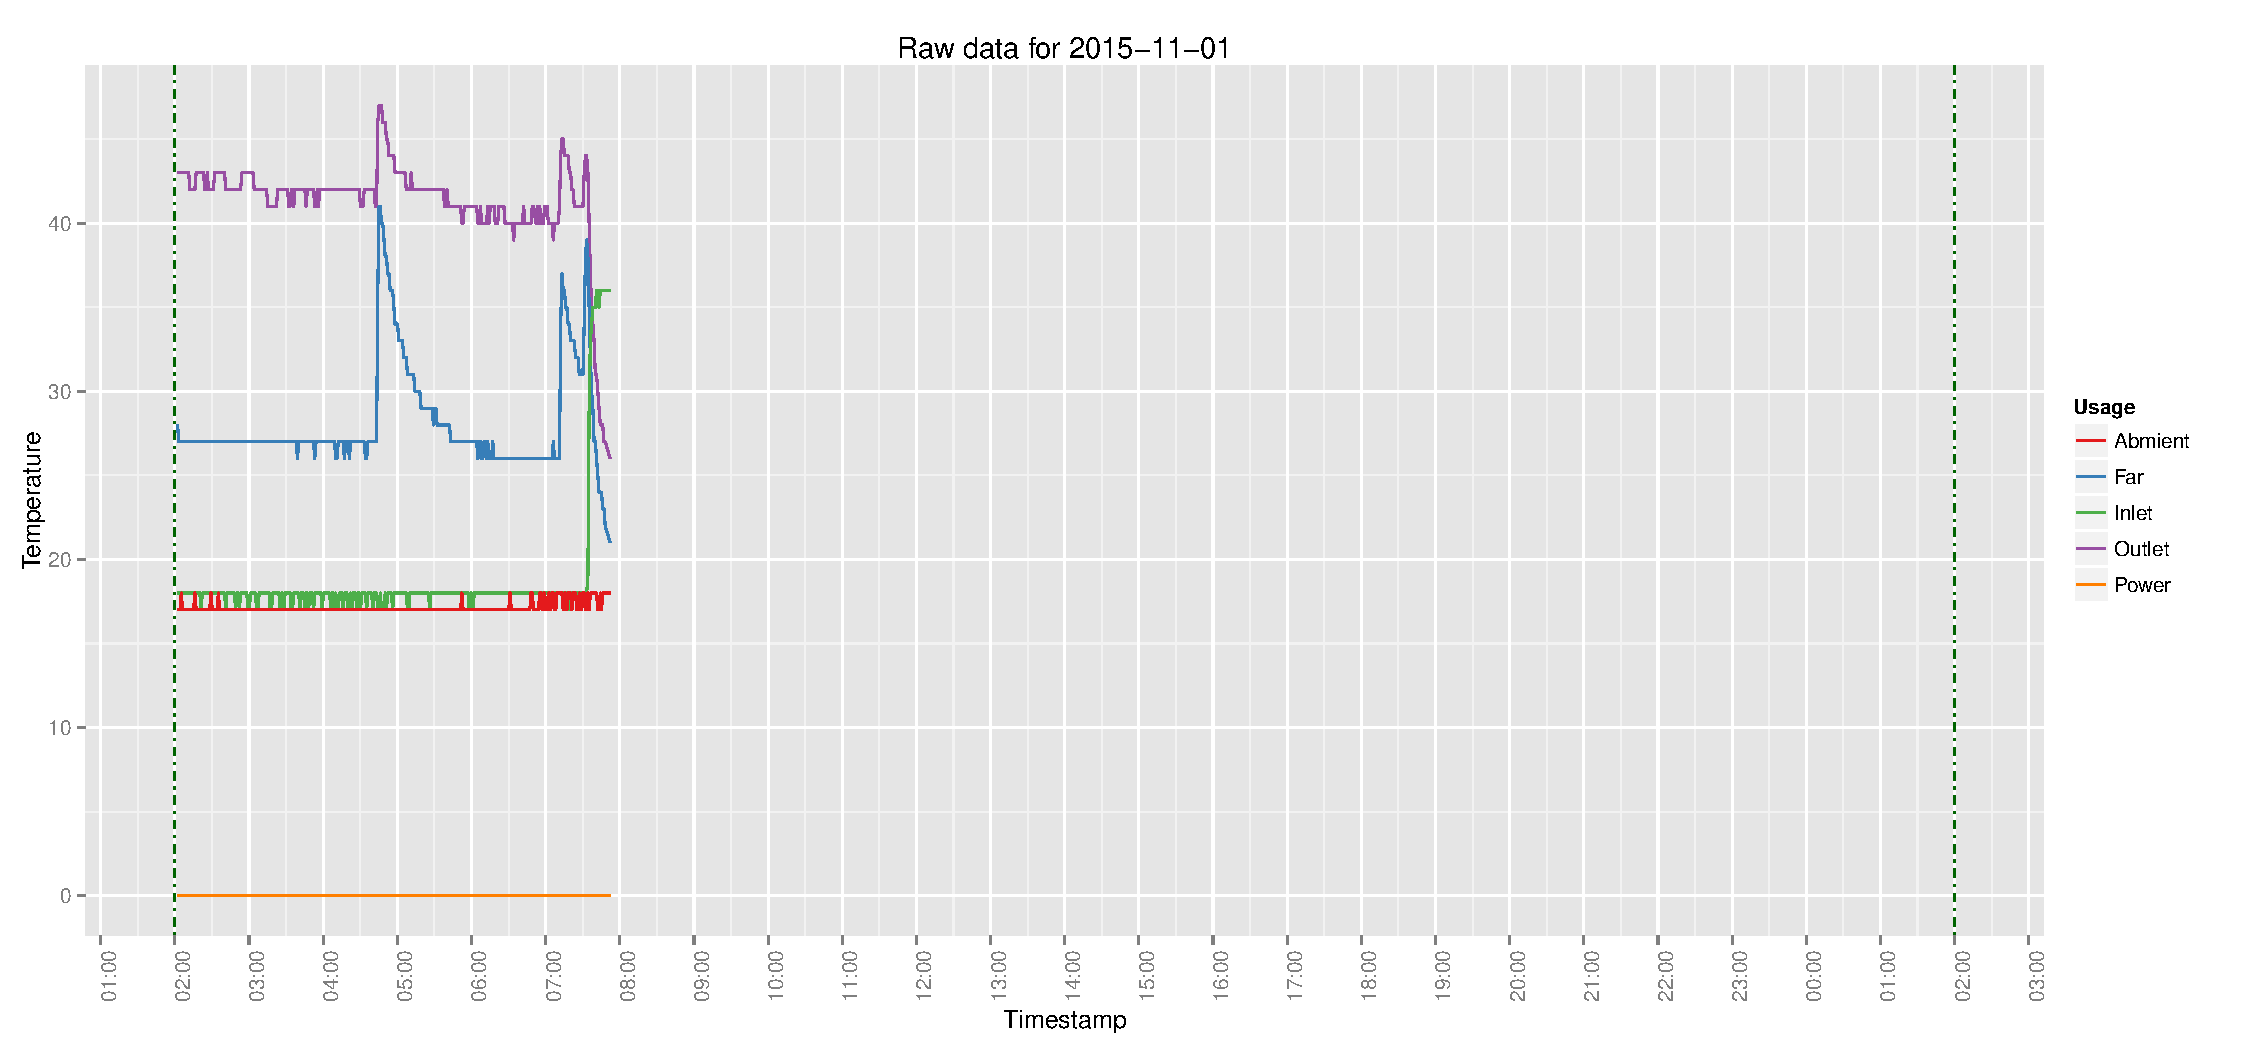
\includegraphics[width=\maxwidth]{figure/raw-1} \caption[Raw data]{Raw data}\label{fig:raw}
\end{figure}


\end{knitrout}




\end{document}
